\documentclass[]{article}
\usepackage{lmodern}
\usepackage{amssymb,amsmath}
\usepackage{ifxetex,ifluatex}
\usepackage{fixltx2e} % provides \textsubscript
\ifnum 0\ifxetex 1\fi\ifluatex 1\fi=0 % if pdftex
  \usepackage[T1]{fontenc}
  \usepackage[utf8]{inputenc}
\else % if luatex or xelatex
  \ifxetex
    \usepackage{mathspec}
  \else
    \usepackage{fontspec}
  \fi
  \defaultfontfeatures{Ligatures=TeX,Scale=MatchLowercase}
\fi
% use upquote if available, for straight quotes in verbatim environments
\IfFileExists{upquote.sty}{\usepackage{upquote}}{}
% use microtype if available
\IfFileExists{microtype.sty}{%
\usepackage{microtype}
\UseMicrotypeSet[protrusion]{basicmath} % disable protrusion for tt fonts
}{}
\usepackage[margin=1in]{geometry}
\usepackage{hyperref}
\hypersetup{unicode=true,
            pdftitle={Functional data analysis of eye pupil dilation},
            pdfauthor={Paolo Girardi},
            pdfborder={0 0 0},
            breaklinks=true}
\urlstyle{same}  % don't use monospace font for urls
\usepackage{color}
\usepackage{fancyvrb}
\newcommand{\VerbBar}{|}
\newcommand{\VERB}{\Verb[commandchars=\\\{\}]}
\DefineVerbatimEnvironment{Highlighting}{Verbatim}{commandchars=\\\{\}}
% Add ',fontsize=\small' for more characters per line
\usepackage{framed}
\definecolor{shadecolor}{RGB}{248,248,248}
\newenvironment{Shaded}{\begin{snugshade}}{\end{snugshade}}
\newcommand{\AlertTok}[1]{\textcolor[rgb]{0.94,0.16,0.16}{#1}}
\newcommand{\AnnotationTok}[1]{\textcolor[rgb]{0.56,0.35,0.01}{\textbf{\textit{#1}}}}
\newcommand{\AttributeTok}[1]{\textcolor[rgb]{0.77,0.63,0.00}{#1}}
\newcommand{\BaseNTok}[1]{\textcolor[rgb]{0.00,0.00,0.81}{#1}}
\newcommand{\BuiltInTok}[1]{#1}
\newcommand{\CharTok}[1]{\textcolor[rgb]{0.31,0.60,0.02}{#1}}
\newcommand{\CommentTok}[1]{\textcolor[rgb]{0.56,0.35,0.01}{\textit{#1}}}
\newcommand{\CommentVarTok}[1]{\textcolor[rgb]{0.56,0.35,0.01}{\textbf{\textit{#1}}}}
\newcommand{\ConstantTok}[1]{\textcolor[rgb]{0.00,0.00,0.00}{#1}}
\newcommand{\ControlFlowTok}[1]{\textcolor[rgb]{0.13,0.29,0.53}{\textbf{#1}}}
\newcommand{\DataTypeTok}[1]{\textcolor[rgb]{0.13,0.29,0.53}{#1}}
\newcommand{\DecValTok}[1]{\textcolor[rgb]{0.00,0.00,0.81}{#1}}
\newcommand{\DocumentationTok}[1]{\textcolor[rgb]{0.56,0.35,0.01}{\textbf{\textit{#1}}}}
\newcommand{\ErrorTok}[1]{\textcolor[rgb]{0.64,0.00,0.00}{\textbf{#1}}}
\newcommand{\ExtensionTok}[1]{#1}
\newcommand{\FloatTok}[1]{\textcolor[rgb]{0.00,0.00,0.81}{#1}}
\newcommand{\FunctionTok}[1]{\textcolor[rgb]{0.00,0.00,0.00}{#1}}
\newcommand{\ImportTok}[1]{#1}
\newcommand{\InformationTok}[1]{\textcolor[rgb]{0.56,0.35,0.01}{\textbf{\textit{#1}}}}
\newcommand{\KeywordTok}[1]{\textcolor[rgb]{0.13,0.29,0.53}{\textbf{#1}}}
\newcommand{\NormalTok}[1]{#1}
\newcommand{\OperatorTok}[1]{\textcolor[rgb]{0.81,0.36,0.00}{\textbf{#1}}}
\newcommand{\OtherTok}[1]{\textcolor[rgb]{0.56,0.35,0.01}{#1}}
\newcommand{\PreprocessorTok}[1]{\textcolor[rgb]{0.56,0.35,0.01}{\textit{#1}}}
\newcommand{\RegionMarkerTok}[1]{#1}
\newcommand{\SpecialCharTok}[1]{\textcolor[rgb]{0.00,0.00,0.00}{#1}}
\newcommand{\SpecialStringTok}[1]{\textcolor[rgb]{0.31,0.60,0.02}{#1}}
\newcommand{\StringTok}[1]{\textcolor[rgb]{0.31,0.60,0.02}{#1}}
\newcommand{\VariableTok}[1]{\textcolor[rgb]{0.00,0.00,0.00}{#1}}
\newcommand{\VerbatimStringTok}[1]{\textcolor[rgb]{0.31,0.60,0.02}{#1}}
\newcommand{\WarningTok}[1]{\textcolor[rgb]{0.56,0.35,0.01}{\textbf{\textit{#1}}}}
\usepackage{graphicx,grffile}
\makeatletter
\def\maxwidth{\ifdim\Gin@nat@width>\linewidth\linewidth\else\Gin@nat@width\fi}
\def\maxheight{\ifdim\Gin@nat@height>\textheight\textheight\else\Gin@nat@height\fi}
\makeatother
% Scale images if necessary, so that they will not overflow the page
% margins by default, and it is still possible to overwrite the defaults
% using explicit options in \includegraphics[width, height, ...]{}
\setkeys{Gin}{width=\maxwidth,height=\maxheight,keepaspectratio}
\IfFileExists{parskip.sty}{%
\usepackage{parskip}
}{% else
\setlength{\parindent}{0pt}
\setlength{\parskip}{6pt plus 2pt minus 1pt}
}
\setlength{\emergencystretch}{3em}  % prevent overfull lines
\providecommand{\tightlist}{%
  \setlength{\itemsep}{0pt}\setlength{\parskip}{0pt}}
\setcounter{secnumdepth}{0}
% Redefines (sub)paragraphs to behave more like sections
\ifx\paragraph\undefined\else
\let\oldparagraph\paragraph
\renewcommand{\paragraph}[1]{\oldparagraph{#1}\mbox{}}
\fi
\ifx\subparagraph\undefined\else
\let\oldsubparagraph\subparagraph
\renewcommand{\subparagraph}[1]{\oldsubparagraph{#1}\mbox{}}
\fi

%%% Use protect on footnotes to avoid problems with footnotes in titles
\let\rmarkdownfootnote\footnote%
\def\footnote{\protect\rmarkdownfootnote}

%%% Change title format to be more compact
\usepackage{titling}

% Create subtitle command for use in maketitle
\providecommand{\subtitle}[1]{
  \posttitle{
    \begin{center}\large#1\end{center}
    }
}

\setlength{\droptitle}{-2em}

  \title{Functional data analysis of eye pupil dilation}
    \pretitle{\vspace{\droptitle}\centering\huge}
  \posttitle{\par}
    \author{Paolo Girardi}
    \preauthor{\centering\large\emph}
  \postauthor{\par}
      \predate{\centering\large\emph}
  \postdate{\par}
    \date{26/11/2019}


\begin{document}
\maketitle

\newcommand{\normb}[1]{\bigl\|{#1}\bigr\|}
\newcommand{\Ind}[1]{\mbox{\larger\textbf{1}}_{#1}}
\newcommand{\tr}{{}^{\intercal}}
\newcommand{\balpha}{\boldsymbol{\alpha}}
\newcommand{\bbeta}{\boldsymbol{\beta}}
\newcommand{\btheta}{\boldsymbol{\theta}}
\newcommand{\bgamma}{\boldsymbol{\gamma}}
\newcommand{\bdelta}{\boldsymbol{\delta}}
\newcommand{\bpsi}{\boldsymbol{\psi}}
\newcommand{\bTheta}{\boldsymbol{\Theta}}
\newcommand{\bB}{\mathbf{B}}
\newcommand{\bX}{\mathbf{X}}
\newcommand{\bY}{\mathbf{Y}}
\newcommand{\bZ}{\mathbf{Z}}
\newcommand{\ba}{\mathbf{a}}
\newcommand{\bc}{\mathbf{c}}
\newcommand{\bu}{\mathbf{u}}
\newcommand{\bv}{\mathbf{v}}
\newcommand{\bw}{\mathbf{w}}
\newcommand{\bx}{\mathbf{x}}
\newcommand{\by}{\mathbf{y}}
\newcommand{\bz}{\mathbf{z}}

\abstract

In general, methods for correlating pupillary response to the cognitive
activity of a subject undergoing an evaluation of cognitive activity are
based on average values or analysis of peak activity.

However, in this type of analysis, we lose the temporal form of the data
which is a valuable feature because of temporal scale (high temporal
scale 250 Hz) or specific trend pattern Eye tracking data contains
several features:

\begin{itemize}
\item Eye point of gaze;
\item Fixation (and relative Area Of Interest -AOI-) and Saccade time periods.
\item \textbf{Eye pupil dilation}
\end{itemize}

Differently by the classical approach based on differences on
``averaged'' values over a certain period, we propose a functional
clustering model that takes into account the entire behaviour of a eye
dilation time series.

\section{Functional data clustering... a gentle introduction}

The statistical problem is to cluster subjects with common temporal
behaviour regarding their eye dilation. Let
\(\mathbf{Y}_i = (Y_i (t_{i,1}),\ldots,Y_i (t_{i,m_i}))'\) a time series
of \(m_i\) values collected for the subject \(s_i\), \(i=1,\ldots,n\).
The value \(m_i\) corresponds to the number of observations included in
the \(i-th\) time series. We suppose to observe \(n\) time series and we
want to cluster them in \(C\) clusters.

\subsection{Model-based Functional data clustering}

In a mixture-model based approach to clustering the cluster membership
of the i-th time seriesis represented by a latent random vector
\(\mathbf{Z}_i=(Z_{i,1},\ldots,Z_{i,C})'\), where \(Z_{i,c}=1\) if the
time series belongs to the cluster \(c\),\(Z_{i,c}=0\) otherwise. Then a
model for the complete data \((\mathbf{Y}_i,\mathbf{Z}_i)\),
\(i=1,\ldots,n\) is specified in a hierarchical way. Suppose that the
\(i\)-th time series belongs to the cluster \(c\), i.e.~\(Z_{i,c}=1\)
and \(Z_{i,c'}=0\) forc'\(\ne\) c.

Given the cluster membership \(\mathbf{Z}_i\),we suppose that
\(\mathbf{Y}_i\)is a discrete and noised measurement of a smooth
time-varying curve \(f_{c}(t)\), namely \[
Y_i(t_{i,j})=f_c(t_{i,j})+\varepsilon_{i}(t_{i,j}),\qquad j=1,\ldots,m_i.
\] The smooth function \(f_c(t)\) is described by a linear combination
of \(K\) B-spline basis functions \(B_k(t)\), \(k=1,\ldots,K\),
evaluated at \(K-1\) equally spaced in knots, namely \[
f_c(t)=\sum_{k=1}^K \psi_{c,k} B_k(t)
=\gamma^\top B(x)
\] where \(\boldsymbol{\psi}_{c}=(\psi_{c,1},\ldots, \psi_{c,K})'\) is a
vector of unknown parameters.

In view of our application, it does not seem too restrictive to assume
that \(\varepsilon_i(t_{i,j})\) are temporally independent Gaussian
random errors with zero mean and cluster specific variance
\(\sigma_c^2\). It turns out that time series
\(\mathbf{Y}_1,\ldots,\mathbf{Y}_n\) are conditionally independent on
\(\mathbf{Z}_1,\ldots,\mathbf{Z}_n\) and \begin{equation}\label{eq:mod}
Y_i(t_{i,j})|\mathbf{Z}_{i} \sim \mathcal{N}\left(\sum_{k=1}^K \psi_{c,k} B_k(t_{i,j}),\sigma^2_c\right), \quad j=1\ldots,m_i.
 \end{equation}

\subsection{Two steps Functional data clustering}

A second different approach called ``2 steps - clustering'' we performed
an unsupervised classification based on measures of the distance between
the 2 curves. we calculated a distance matrix, based on the L2 norm
between two estimated curves \(i\) and \(j\)
\(f_i(t)=\sum_{k=1}^K \psi_{i,k} B_k(t)\) and
\(f_j(t)=\sum_{k=1}^K \psi_{j,k} B_k(t)\) is calculated as following:
\begin{equation}\label{eq:2stepsfun}
d_{i,j}= \sqrt{(\sum_{k=1}^K \psi_{i,k} B_k(t)-\sum_{k=1}^K \psi_{j,k} B_k(t))^2 }\approx \sqrt{\sum_{k=1}^K (\psi_{i,k}-\psi_{j,k})^2}  \mbox{   } \forall i \neq j,
 \end{equation} where \(d_{i_j}\) is an element of distance matrix \(D\)
based on the euclidean distance. We applied to the distance matrix an
algorithm in order to cluster toghether similar curves. A summary of the
statistical methods proposed for functional data clustering is reported
in a review of (Jacques and Preda
\protect\hyperlink{ref-jacques2014}{2014}) reported in the following
figure.

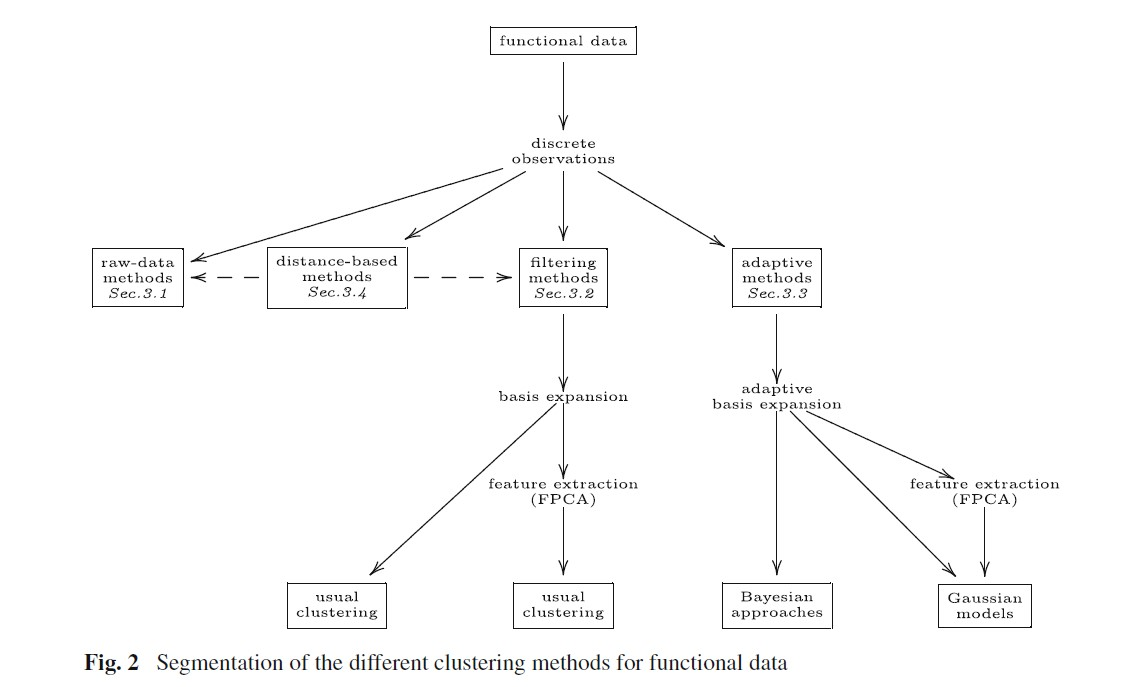
\includegraphics{fig2_preda.jpg}

\section{Eye tracking dilation dataset}

We consider a dataset formed by pupil eye dilation records of 25 female
childs involved in two trials consisting in the visualization of three
images for a total of 18 seconds differing between them only for the
ending scene:

\begin{itemize}
\item Trial 1: Ambiguous situation - Teacher with bad reaction - \textbf{Child with bad reaction};
\item Trial 2: Ambiguous situation - Teacher with bad reaction - \textbf{Child with mild reaction}.
\end{itemize}

\begin{tabular}{cccc}
\textbf{Trial 1}& 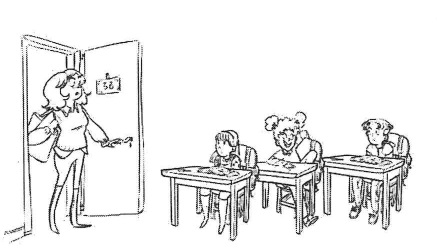
\includegraphics[width=0.25\textwidth]{ambigua.jpg} & 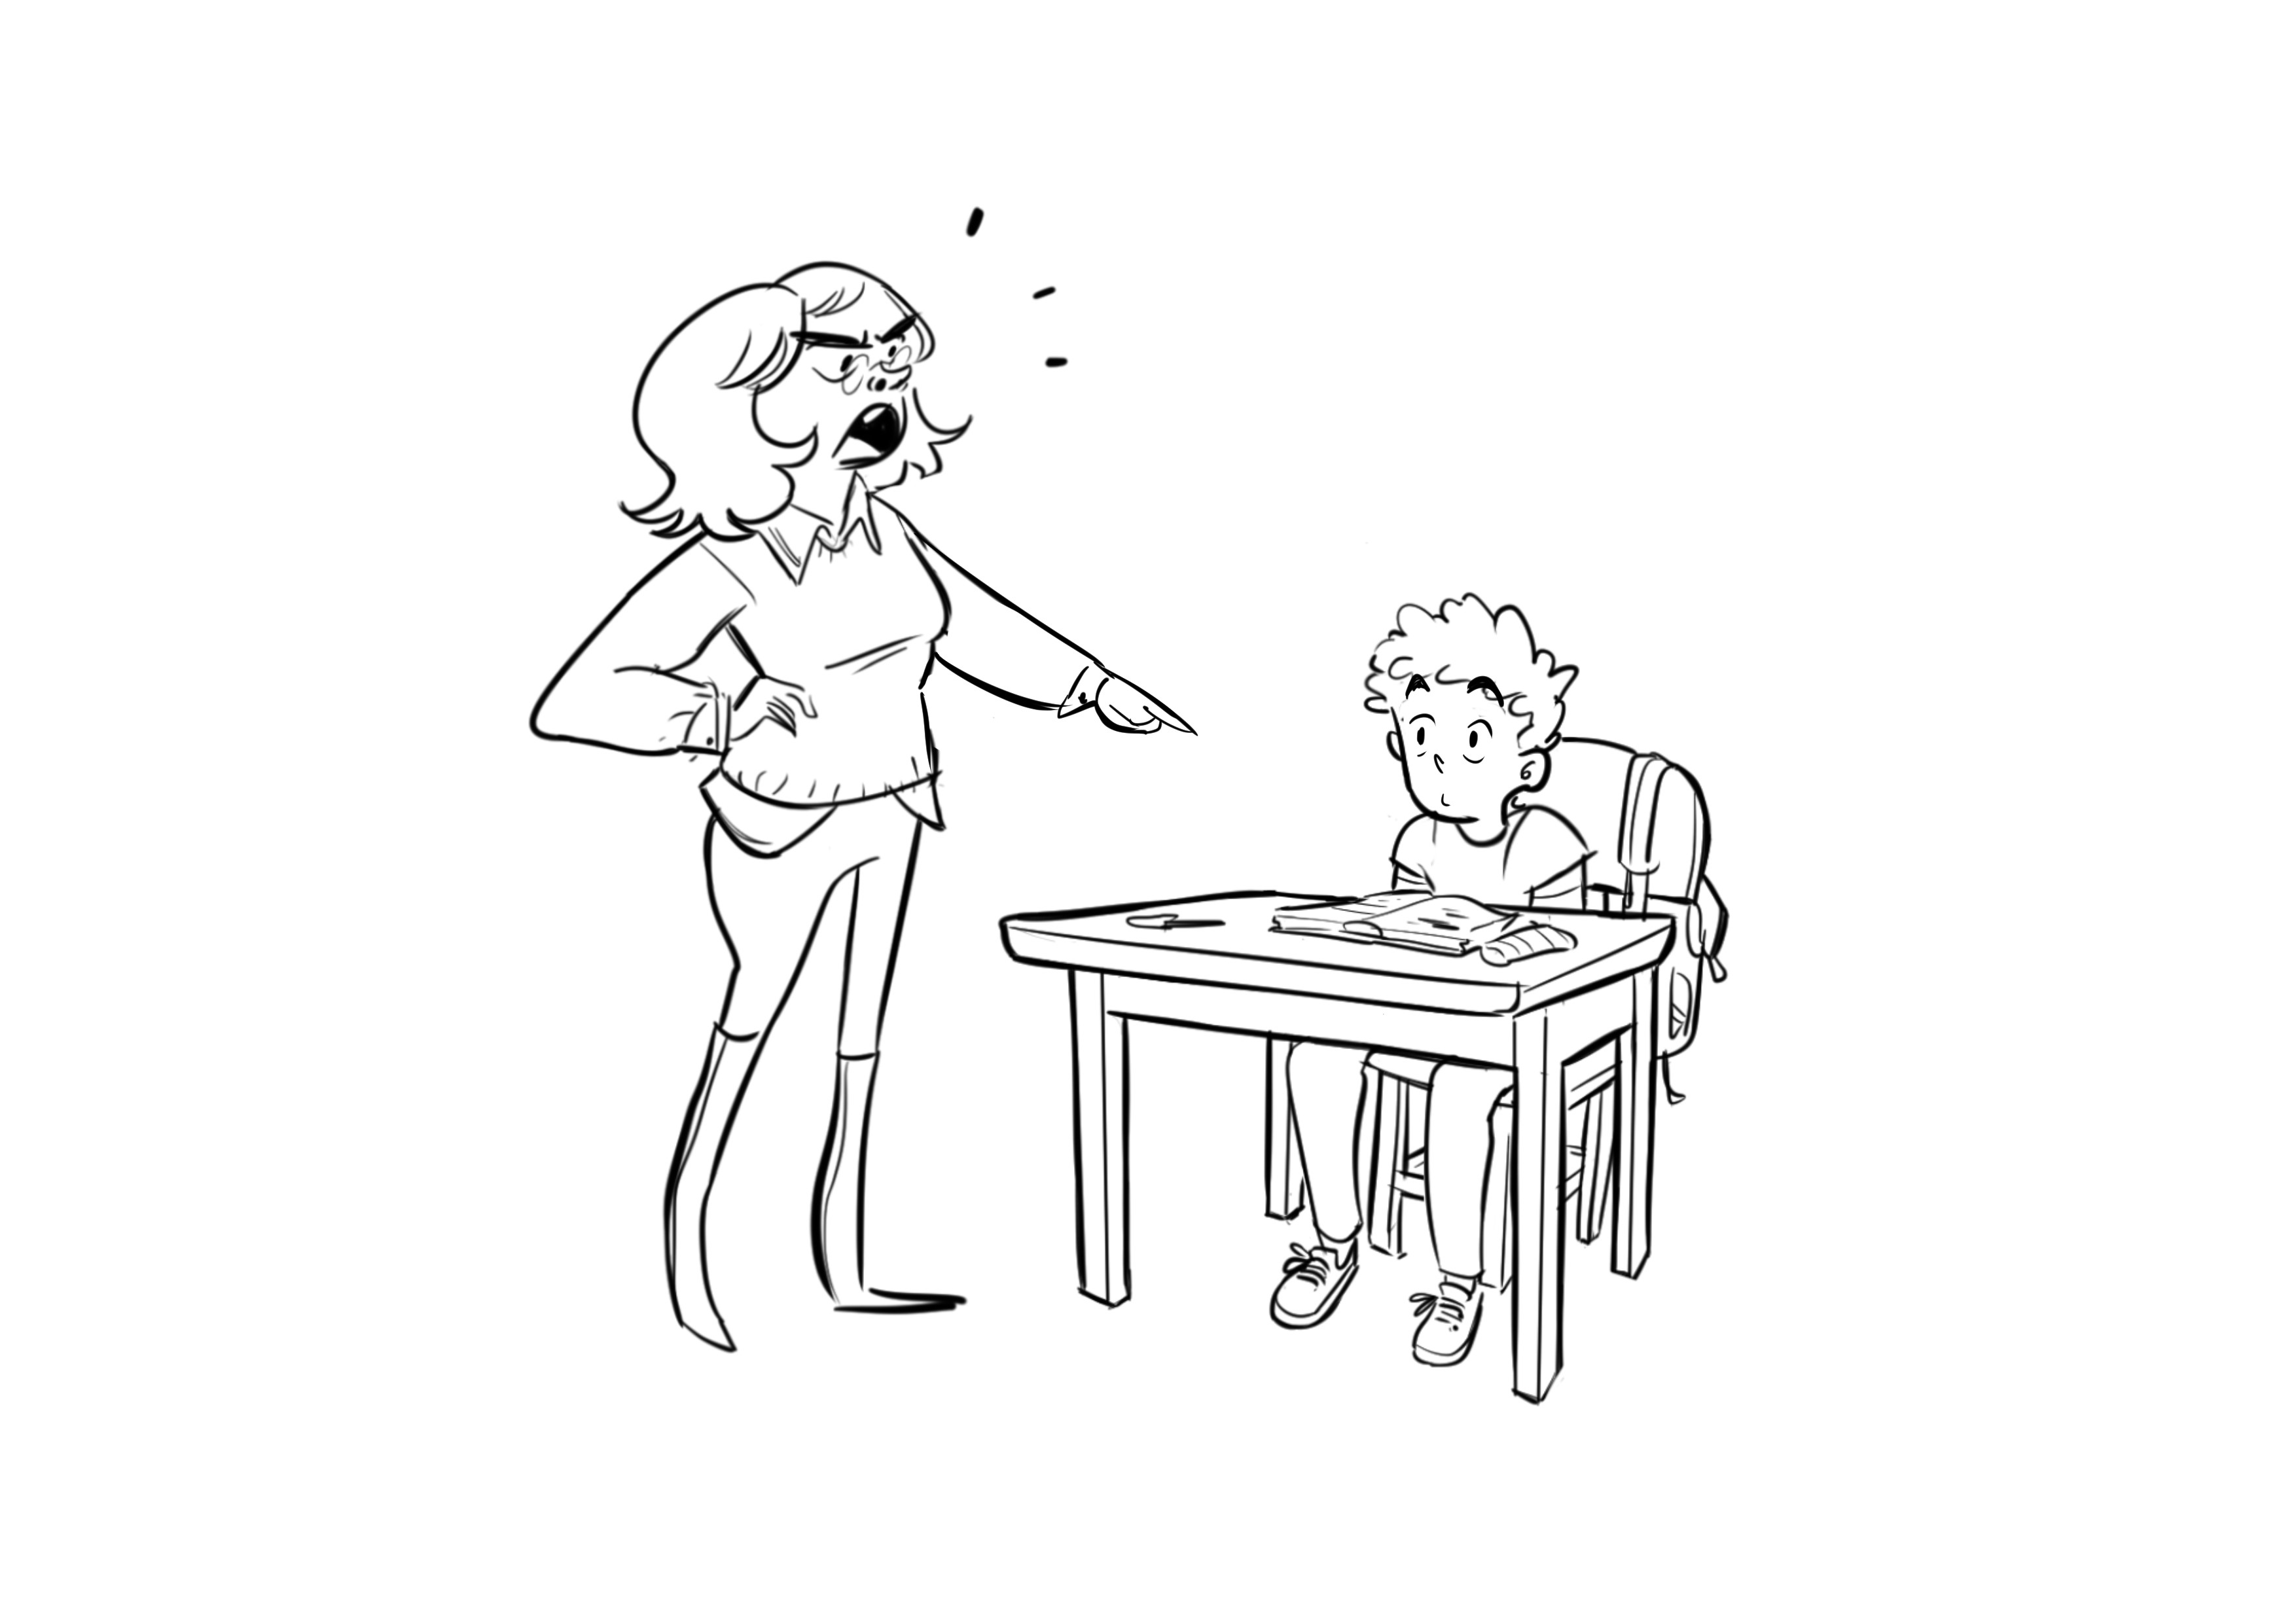
\includegraphics[width=0.25\textwidth]{maestra cattiva.jpg}& 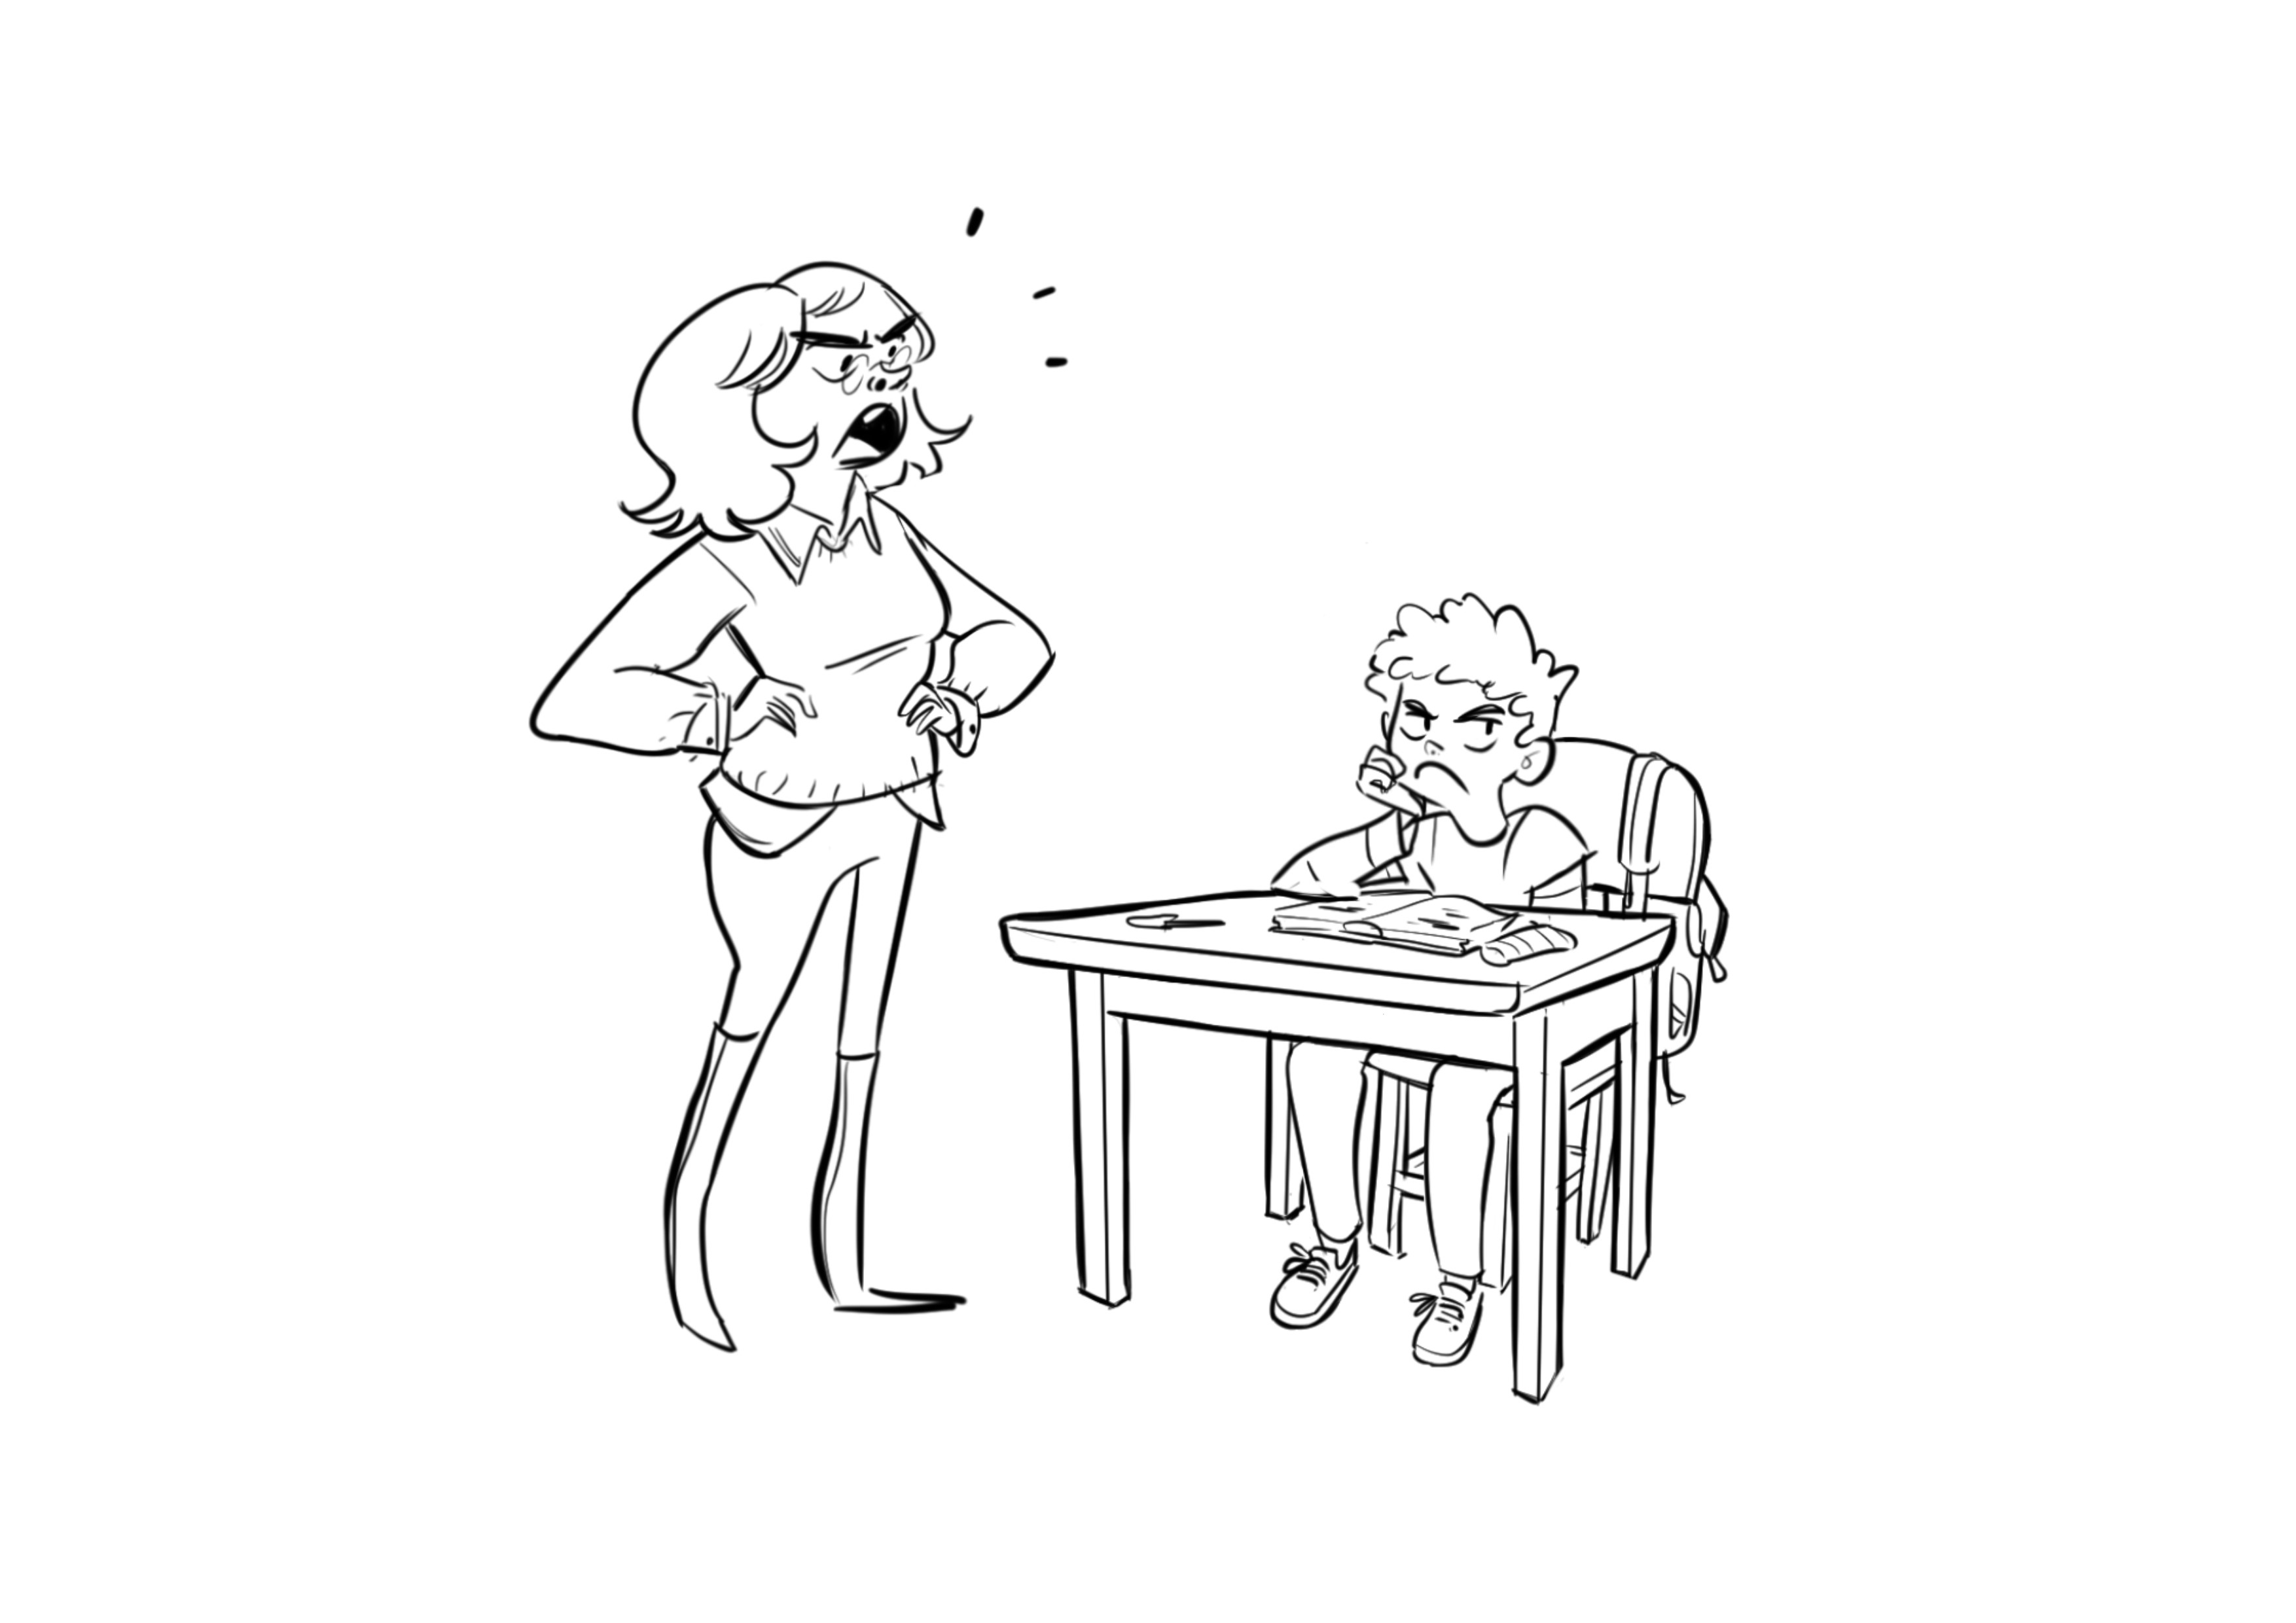
\includegraphics[width=0.25\textwidth]{maestra-ostile-bambino-ostile.jpg}\\
\textbf{Trial 2}& 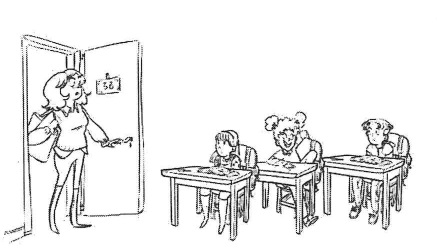
\includegraphics[width=0.25\textwidth]{ambigua.jpg} &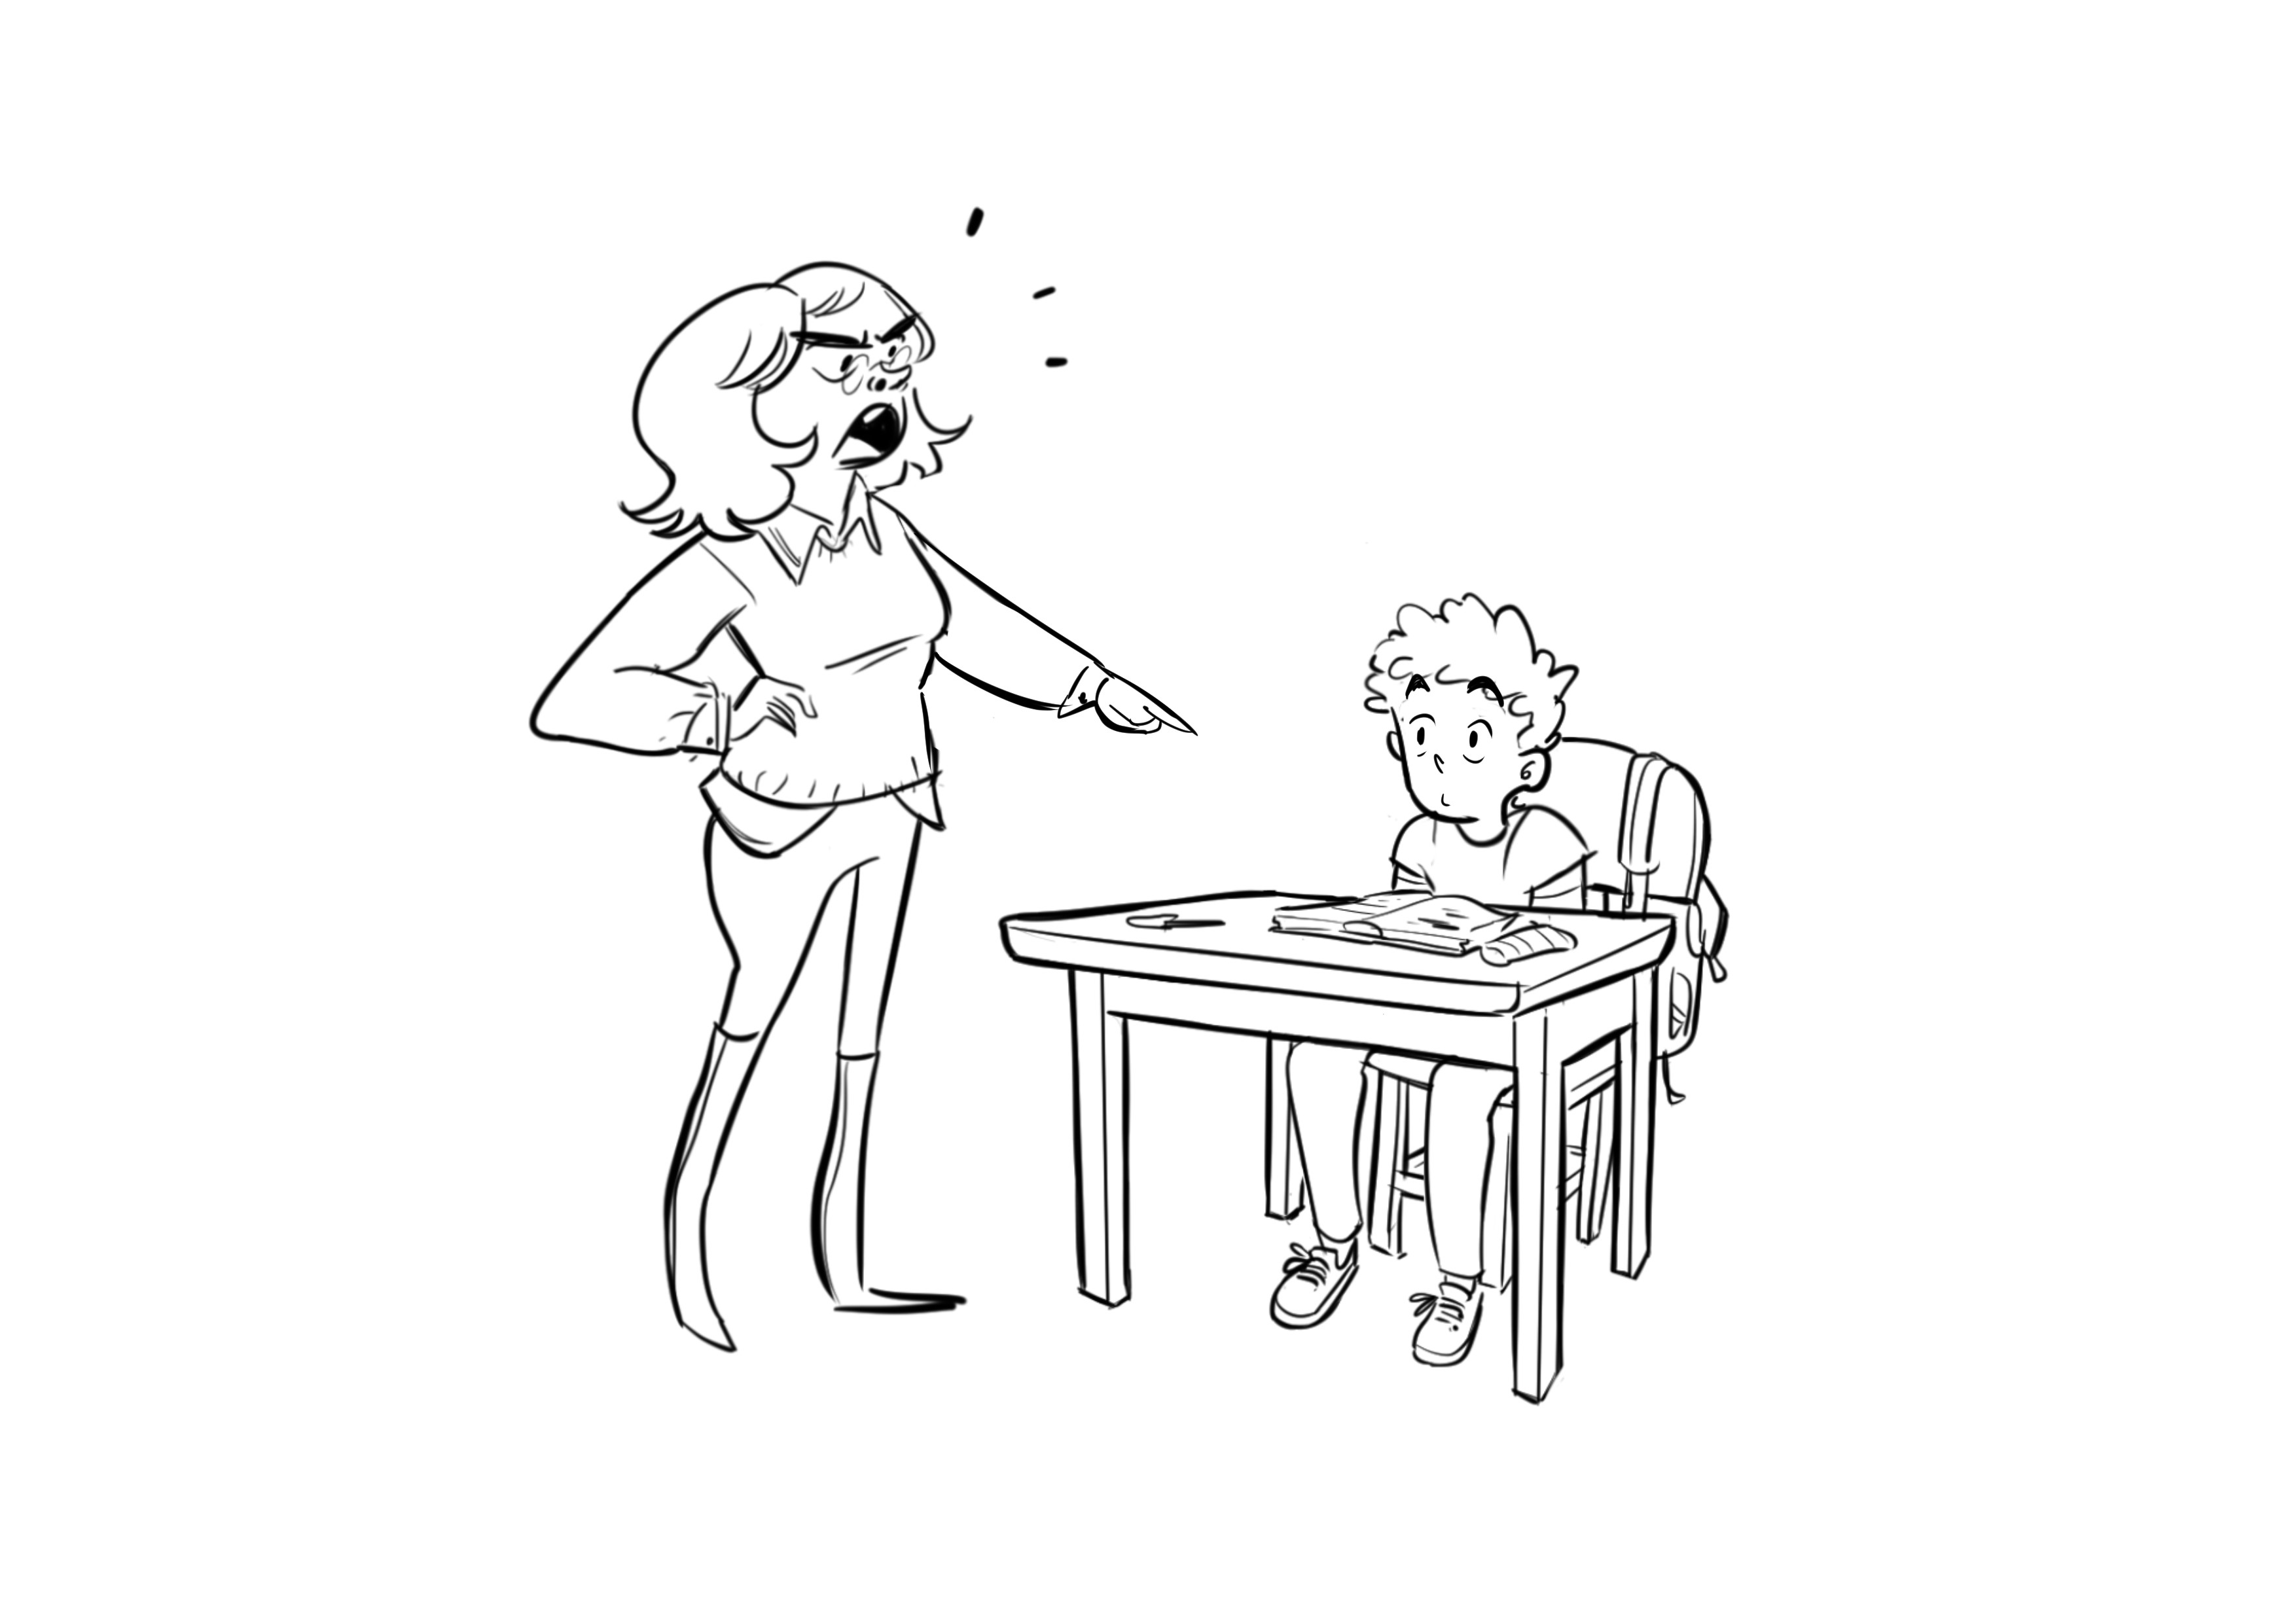
\includegraphics[width=0.25\textwidth]{maestra cattiva.jpg} & 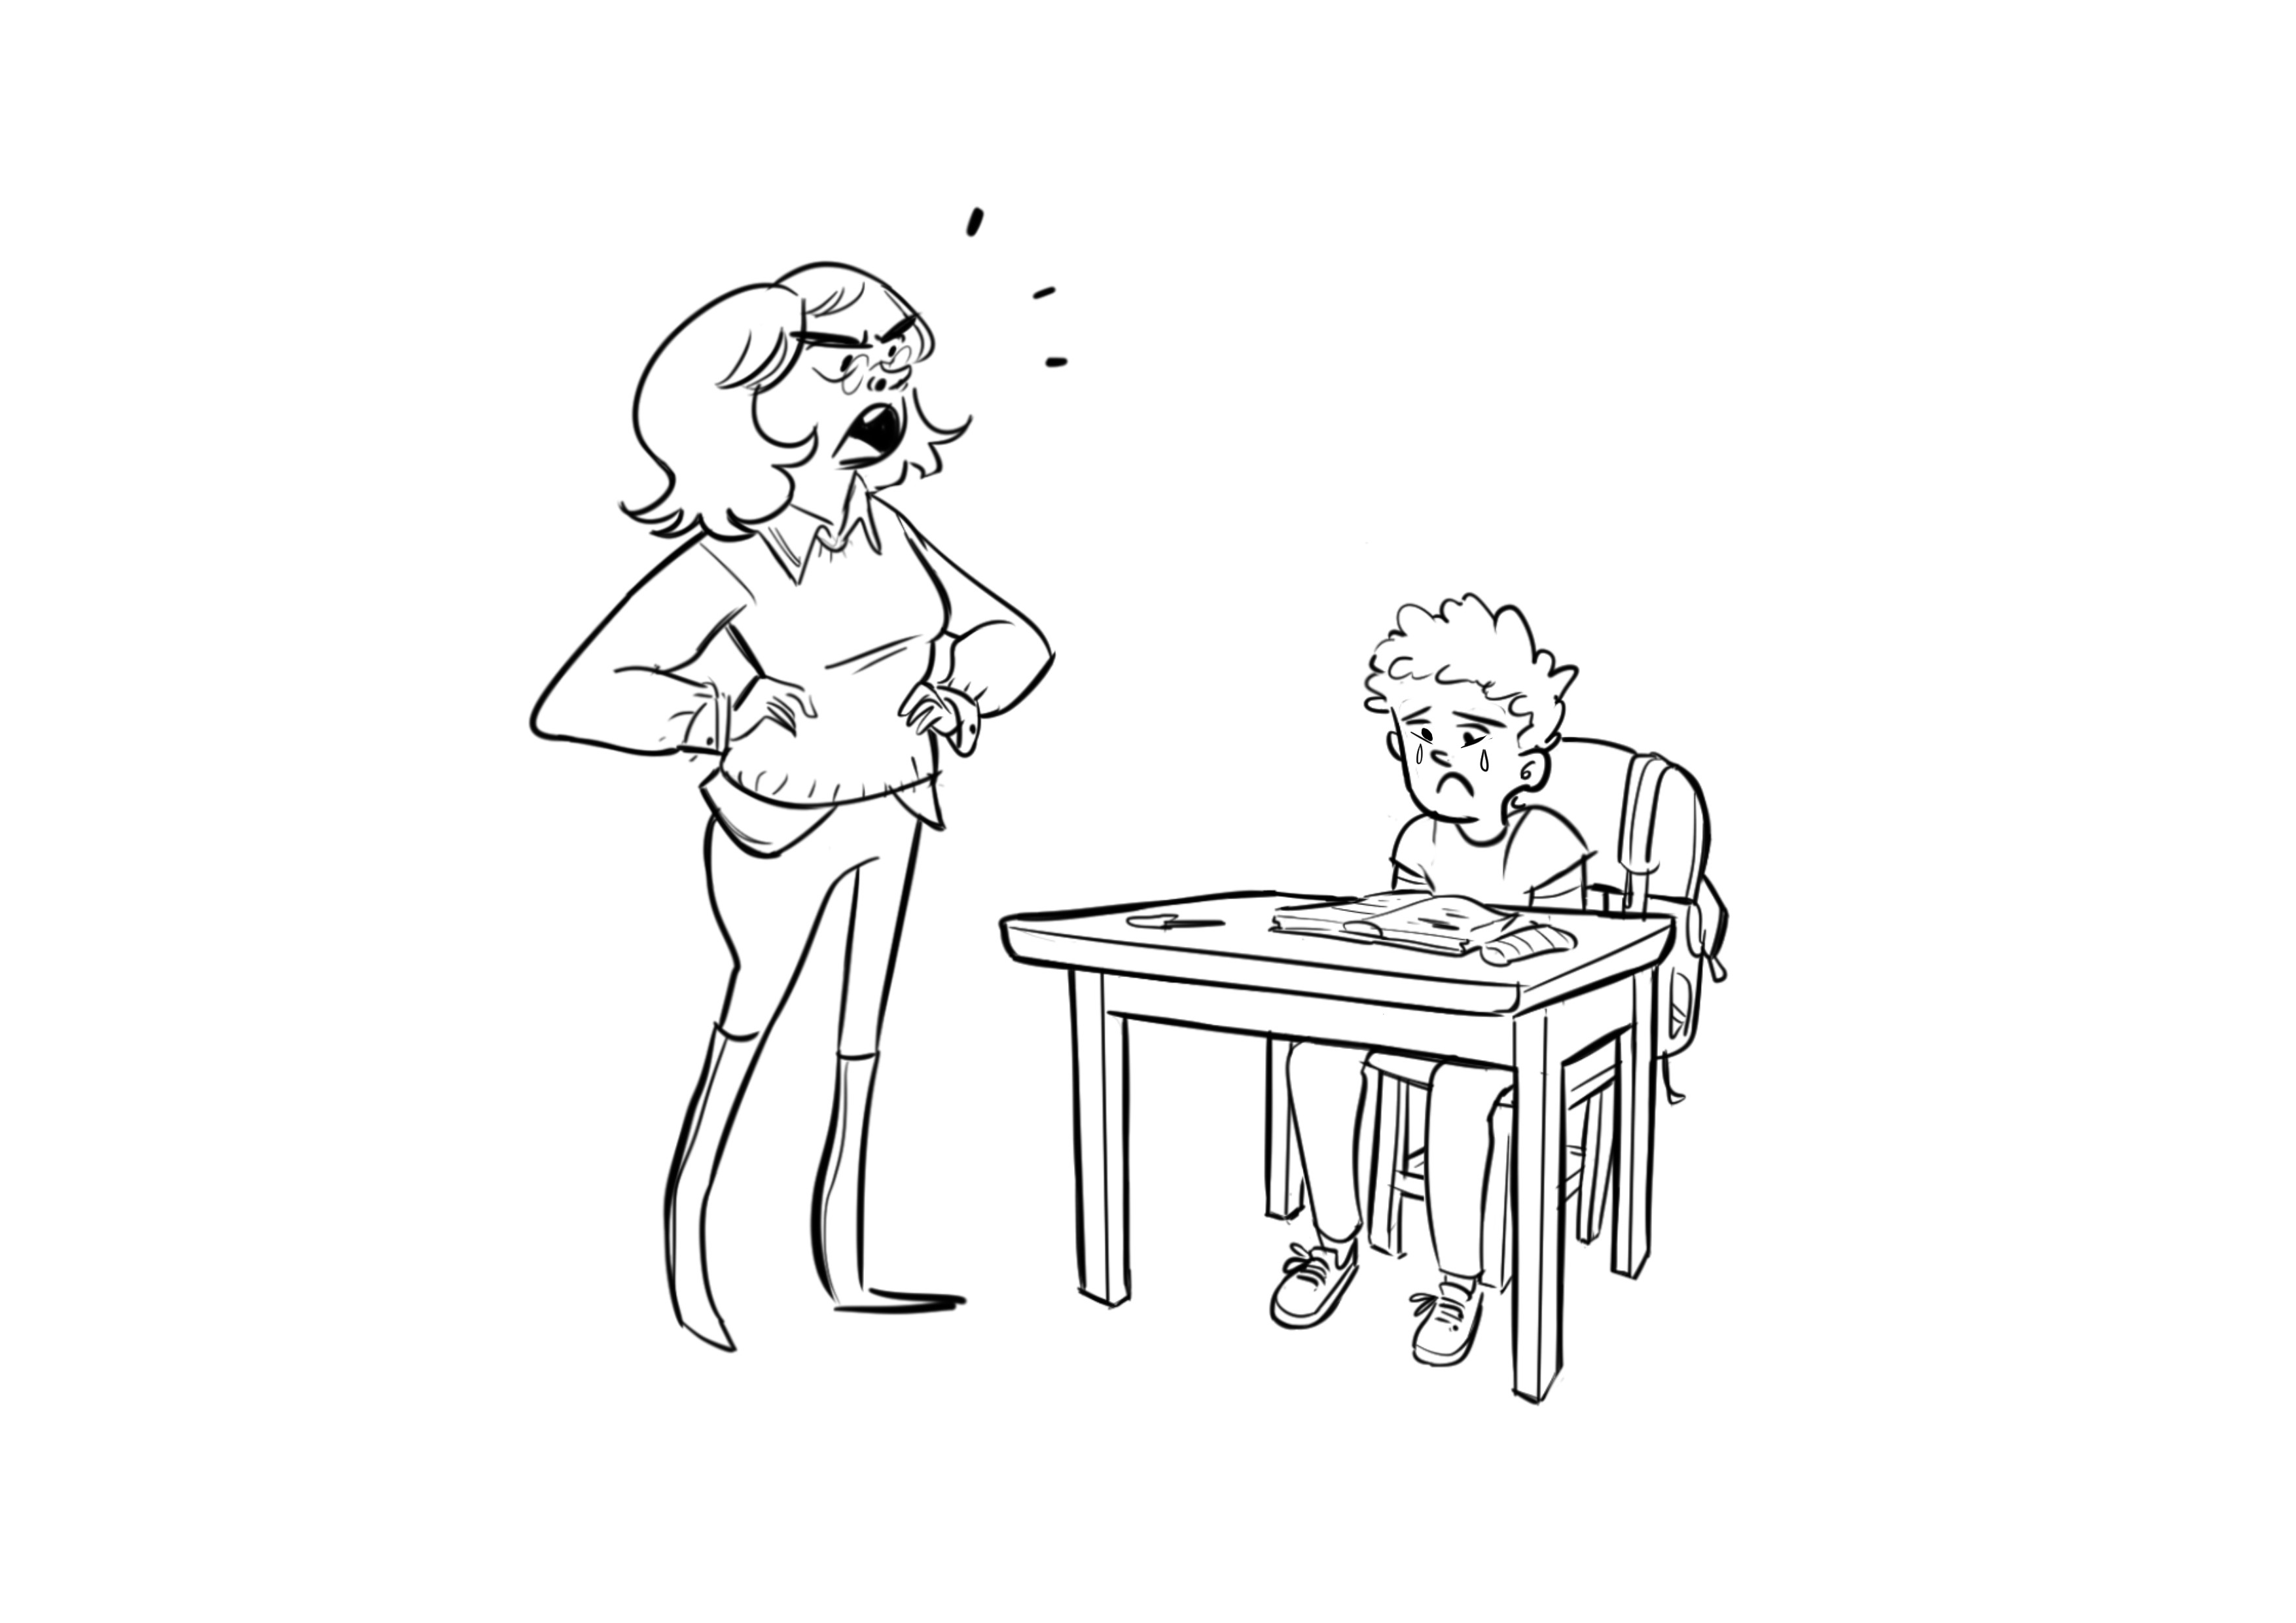
\includegraphics[width=0.25\textwidth]{maestra-ostile-bambino-buono.jpg}\\
\end{tabular}

\begin{Shaded}
\begin{Highlighting}[]
\KeywordTok{rm}\NormalTok{(}\DataTypeTok{list=}\KeywordTok{ls}\NormalTok{())}
\KeywordTok{setwd}\NormalTok{(}\StringTok{"C:/Users/utente/Desktop/Eye_tracker/"}\NormalTok{)}
\CommentTok{### data are preprocessed (time series with 0 mean and unit standard deviation)}
\NormalTok{db_tf1<-}\KeywordTok{read.csv}\NormalTok{(}\StringTok{"trial1_f.csv"}\NormalTok{)}
\NormalTok{db_tf2<-}\KeywordTok{read.csv}\NormalTok{(}\StringTok{"trial2_f.csv"}\NormalTok{)}
\CommentTok{#imported variables}
\KeywordTok{names}\NormalTok{(db_tf1)}
\end{Highlighting}
\end{Shaded}

\begin{verbatim}
##  [1] "X"      "sex"    "id"     "test"   "img"    "time"   "id_f"  
##  [8] "id_s"   "type"   "durata" "p_sx"   "p_dx"   "v_sx"   "v_dx"
\end{verbatim}

\begin{Shaded}
\begin{Highlighting}[]
\CommentTok{# p_sx and d_sx are Right and Left eye dilations}
\CommentTok{# time is the temporal scale}
\CommentTok{# id is the subject ID}
\KeywordTok{table}\NormalTok{(db_tf1}\OperatorTok{$}\NormalTok{id)}
\end{Highlighting}
\end{Shaded}

\begin{verbatim}
## 
## F1301 F1318 F1322 F1326 F1340  F213  F215  F216  F243  F245  F248  F249 
##  1083  1084  1082  1082  1082  1083  1084  1080  1083  1083  1083  1083 
##  F252  F257  F260  F266  F273  F282  F286  F288  F290  F292  F295  F296 
##  1084  1085  1084  1082  1084  1082  1084  1083  1082  1082  1085  1084 
##  F299 
##  1082
\end{verbatim}

\begin{Shaded}
\begin{Highlighting}[]
\CommentTok{###more than 1000 time points for each time series (18/1082= 0.017s time scale)}
\CommentTok{### but different time points }
\KeywordTok{length}\NormalTok{(}\KeywordTok{table}\NormalTok{(db_tf1}\OperatorTok{$}\NormalTok{time))}
\end{Highlighting}
\end{Shaded}

\begin{verbatim}
## [1] 6948
\end{verbatim}

\begin{Shaded}
\begin{Highlighting}[]
\CommentTok{## Marginal distribution ofRight and Left eye dilations}
\KeywordTok{boxplot}\NormalTok{(db_tf1}\OperatorTok{$}\NormalTok{p_dx,db_tf1}\OperatorTok{$}\NormalTok{p_sx)}
\CommentTok{## Right and Left eye dilations are highly correlated}
\KeywordTok{cor.test}\NormalTok{(db_tf1}\OperatorTok{$}\NormalTok{p_dx,db_tf1}\OperatorTok{$}\NormalTok{p_sx)}
\end{Highlighting}
\end{Shaded}

\begin{verbatim}
## 
##  Pearson's product-moment correlation
## 
## data:  db_tf1$p_dx and db_tf1$p_sx
## t = 385.96, df = 24860, p-value < 2.2e-16
## alternative hypothesis: true correlation is not equal to 0
## 95 percent confidence interval:
##  0.9239338 0.9274899
## sample estimates:
##       cor 
## 0.9257323
\end{verbatim}

\begin{Shaded}
\begin{Highlighting}[]
\CommentTok{### create the average dilation between two eye}
\NormalTok{db_tf1}\OperatorTok{$}\NormalTok{p<-}\KeywordTok{apply}\NormalTok{(}\KeywordTok{cbind}\NormalTok{(db_tf1}\OperatorTok{$}\NormalTok{p_dx,db_tf1}\OperatorTok{$}\NormalTok{p_sx),}\DecValTok{1}\NormalTok{,mean,}\DataTypeTok{na.rm=}\NormalTok{T)}
\NormalTok{db_tf2}\OperatorTok{$}\NormalTok{p<-}\KeywordTok{apply}\NormalTok{(}\KeywordTok{cbind}\NormalTok{(db_tf2}\OperatorTok{$}\NormalTok{p_dx,db_tf2}\OperatorTok{$}\NormalTok{p_sx),}\DecValTok{1}\NormalTok{,mean,}\DataTypeTok{na.rm=}\NormalTok{T)}




\CommentTok{#some R function to manage plots and data}
\KeywordTok{source}\NormalTok{(}\StringTok{"C:/Users/utente/Desktop/Eye_tracker/functions.R"}\NormalTok{)}
\end{Highlighting}
\end{Shaded}

\begin{verbatim}
## Registered S3 method overwritten by 'xts':
##   method     from
##   as.zoo.xts zoo
\end{verbatim}

\begin{verbatim}
## Registered S3 method overwritten by 'quantmod':
##   method            from
##   as.zoo.data.frame zoo
\end{verbatim}

\begin{verbatim}
## Registered S3 methods overwritten by 'forecast':
##   method             from    
##   fitted.fracdiff    fracdiff
##   residuals.fracdiff fracdiff
\end{verbatim}

\begin{verbatim}
## Loading required package: splines
\end{verbatim}

\begin{verbatim}
## Loading required package: Matrix
\end{verbatim}

\begin{verbatim}
## 
## Attaching package: 'fda'
\end{verbatim}

\begin{verbatim}
## The following object is masked from 'package:graphics':
## 
##     matplot
\end{verbatim}

\includegraphics{FA_psicostat_files/figure-latex/carico intro-1.pdf}

\section{Moving Average Filter}

We need to resample the time series. We apply a Moving Average Filter in
order to get the same time points for each time series as follow:
\[Yfiltered_i(t_{i,j})=\frac{\sum_{i \in W_z} Y_i(t_{i,j}) }{ \# W_z} \]
where \(W_z\) is a time windows and \(\bigcup_{z=1}^{\infty} W_{i}\) is
the entire time window (0-18 seconds)

\begin{Shaded}
\begin{Highlighting}[]
\CommentTok{#set dropping first 2 seconds and endings 5 seconds}
\NormalTok{min<-}\DecValTok{2000}
\NormalTok{max<-}\DecValTok{13000}
\CommentTok{#sampling each time series at 100 ms}
\NormalTok{step<-}\StringTok{ }\KeywordTok{round}\NormalTok{((max}\OperatorTok{-}\NormalTok{min)}\OperatorTok{/}\DecValTok{100}\NormalTok{,}\DecValTok{0}\NormalTok{)}
\CommentTok{# (data vector, subject vector, time vector, time scale, window=(min,max))}
\NormalTok{data_sr1<-}\KeywordTok{sampling_regular}\NormalTok{(db_tf1}\OperatorTok{$}\NormalTok{p,db_tf1}\OperatorTok{$}\NormalTok{id,db_tf1}\OperatorTok{$}\NormalTok{time,step,}\DataTypeTok{window=}\KeywordTok{c}\NormalTok{(min,max))}
\NormalTok{data_sr2<-}\KeywordTok{sampling_regular}\NormalTok{(db_tf2}\OperatorTok{$}\NormalTok{p,db_tf2}\OperatorTok{$}\NormalTok{id,db_tf2}\OperatorTok{$}\NormalTok{time,step,}\DataTypeTok{window=}\KeywordTok{c}\NormalTok{(min,max))}
\CommentTok{# in output a list formed by a matrix of observation and a regularized time vector}

\CommentTok{# MA resampled data for the first child}
\KeywordTok{plot}\NormalTok{(db_tf1}\OperatorTok{$}\NormalTok{time[db_tf1}\OperatorTok{$}\NormalTok{id}\OperatorTok{==}\StringTok{"F1301"} \OperatorTok{&}\StringTok{ }\NormalTok{db_tf1}\OperatorTok{$}\NormalTok{test}\OperatorTok{==}\StringTok{"t1"} \OperatorTok{&}\StringTok{ }\NormalTok{(db_tf1}\OperatorTok{$}\NormalTok{time}\OperatorTok{>}\StringTok{ }\NormalTok{min }\OperatorTok{&}\StringTok{ }\NormalTok{db_tf1}\OperatorTok{$}\NormalTok{time}\OperatorTok{<}\StringTok{ }\NormalTok{max)],}\KeywordTok{scale}\NormalTok{(db_tf1}\OperatorTok{$}\NormalTok{p[db_tf1}\OperatorTok{$}\NormalTok{id}\OperatorTok{==}\StringTok{"F1301"} \OperatorTok{&}\StringTok{ }\NormalTok{db_tf1}\OperatorTok{$}\NormalTok{test}\OperatorTok{==}\StringTok{"t1"} \OperatorTok{&}\StringTok{ }\NormalTok{(db_tf1}\OperatorTok{$}\NormalTok{time}\OperatorTok{>}\StringTok{ }\NormalTok{min }\OperatorTok{&}\StringTok{ }\NormalTok{db_tf1}\OperatorTok{$}\NormalTok{time}\OperatorTok{<}\StringTok{ }\NormalTok{max)],}\DataTypeTok{scale=}\OtherTok{TRUE}\NormalTok{),}\DataTypeTok{type=}\StringTok{"l"}\NormalTok{,}\DataTypeTok{ylab=}\StringTok{"Pupil dilation"}\NormalTok{,}\DataTypeTok{xlab=}\StringTok{"time"}\NormalTok{)}
\KeywordTok{abline}\NormalTok{(}\DataTypeTok{v=}\KeywordTok{c}\NormalTok{(}\DecValTok{5000}\NormalTok{,}\DecValTok{8000}\NormalTok{))}
\KeywordTok{points}\NormalTok{(data_sr1}\OperatorTok{$}\NormalTok{t,data_sr1}\OperatorTok{$}\NormalTok{x_mat[}\DecValTok{1}\NormalTok{,],}\DataTypeTok{pch=}\DecValTok{16}\NormalTok{,}\DataTypeTok{col=}\StringTok{"red"}\NormalTok{)}
\KeywordTok{points}\NormalTok{(data_sr1}\OperatorTok{$}\NormalTok{t,data_sr1}\OperatorTok{$}\NormalTok{x_mat[}\DecValTok{1}\NormalTok{,],}\DataTypeTok{col=}\StringTok{"red"}\NormalTok{,}\DataTypeTok{type=}\StringTok{"l"}\NormalTok{)}
\KeywordTok{legend}\NormalTok{(}\StringTok{"topleft"}\NormalTok{,}\KeywordTok{c}\NormalTok{(}\StringTok{"raw data"}\NormalTok{,}\StringTok{"MA resampled data"}\NormalTok{),}\DataTypeTok{col=}\KeywordTok{c}\NormalTok{(}\DecValTok{1}\NormalTok{,}\DecValTok{2}\NormalTok{),}\DataTypeTok{pch=}\KeywordTok{c}\NormalTok{(}\DecValTok{1}\NormalTok{,}\DecValTok{2}\NormalTok{),}\DataTypeTok{lty=}\KeywordTok{c}\NormalTok{(}\DecValTok{1}\NormalTok{,}\DecValTok{1}\NormalTok{))}
\end{Highlighting}
\end{Shaded}

\includegraphics{FA_psicostat_files/figure-latex/moving average-1.pdf}

\begin{Shaded}
\begin{Highlighting}[]
\CommentTok{#our time series }
\KeywordTok{matplot}\NormalTok{(data_sr1}\OperatorTok{$}\NormalTok{t,}\KeywordTok{t}\NormalTok{(data_sr1}\OperatorTok{$}\NormalTok{x_mat),}\DataTypeTok{type=}\StringTok{"l"}\NormalTok{,}\DataTypeTok{main=}\StringTok{"Trial 1"}\NormalTok{,}\DataTypeTok{ylab=}\StringTok{"Pupil dilation"}\NormalTok{,}\DataTypeTok{xlab=}\StringTok{"time"}\NormalTok{)}
\end{Highlighting}
\end{Shaded}

\includegraphics{FA_psicostat_files/figure-latex/moving average-2.pdf}

\begin{Shaded}
\begin{Highlighting}[]
\KeywordTok{matplot}\NormalTok{(data_sr2}\OperatorTok{$}\NormalTok{t,}\KeywordTok{t}\NormalTok{(data_sr2}\OperatorTok{$}\NormalTok{x_mat),}\DataTypeTok{type=}\StringTok{"l"}\NormalTok{,}\DataTypeTok{main=}\StringTok{"Trial 2"}\NormalTok{,}\DataTypeTok{ylab=}\StringTok{"Pupil dilation"}\NormalTok{,}\DataTypeTok{xlab=}\StringTok{"time"}\NormalTok{)}
\end{Highlighting}
\end{Shaded}

\includegraphics{FA_psicostat_files/figure-latex/moving average-3.pdf}
Lines are overlapping. It is impossibile to observed different time
patterns. It seems hard to discover similar curves. Next step:
Smoothing.

We defined 15 equally distributed knots for the basis of splines. A
number 15 knots seems sufficient. The number of smoothing \(\lambda\) is
chosen by means of the GCV (Generalized Cross validation) criterion.

\begin{Shaded}
\begin{Highlighting}[]
\CommentTok{# we adopt a smoothing strategy, high number of knots (15) }
\CommentTok{# penalizing with L2 norm on second derivatives of coefficients}
\CommentTok{# GCV criterion to select the best lambda }

\NormalTok{l<-}\KeywordTok{exp}\NormalTok{(}\KeywordTok{seq}\NormalTok{(}\DecValTok{10}\NormalTok{,}\DecValTok{20}\NormalTok{,}\FloatTok{0.25}\NormalTok{))}

\NormalTok{gcv1<-}\OtherTok{NULL}
\ControlFlowTok{for}\NormalTok{(i }\ControlFlowTok{in} \DecValTok{1}\OperatorTok{:}\KeywordTok{length}\NormalTok{(l))\{}
\NormalTok{gcv1<-}\KeywordTok{c}\NormalTok{(gcv1,}\KeywordTok{fun_register}\NormalTok{(data_sr1,}\DataTypeTok{lambda=}\NormalTok{l[i], }\DataTypeTok{knots=}\DecValTok{15}\NormalTok{,}\DataTypeTok{plot=}\OtherTok{FALSE}\NormalTok{,}\DataTypeTok{register=}\OtherTok{FALSE}\NormalTok{)}\OperatorTok{$}\NormalTok{gcv)}
\NormalTok{\}}
\NormalTok{graphics}\OperatorTok{::}\KeywordTok{plot}\NormalTok{(gcv1,}\DataTypeTok{ylab=}\StringTok{"GCV"}\NormalTok{,}\DataTypeTok{xlab=}\StringTok{"lambda value"}\NormalTok{)}
\end{Highlighting}
\end{Shaded}

\includegraphics{FA_psicostat_files/figure-latex/smooth-1.pdf}

\begin{Shaded}
\begin{Highlighting}[]
\KeywordTok{which.min}\NormalTok{(gcv1)}
\end{Highlighting}
\end{Shaded}

\begin{verbatim}
## [1] 19
\end{verbatim}

\begin{Shaded}
\begin{Highlighting}[]
\NormalTok{gcv2<-}\OtherTok{NULL}
\ControlFlowTok{for}\NormalTok{(i }\ControlFlowTok{in} \DecValTok{1}\OperatorTok{:}\KeywordTok{length}\NormalTok{(l))\{}
\NormalTok{gcv2<-}\KeywordTok{c}\NormalTok{(gcv2,}\KeywordTok{fun_register}\NormalTok{(data_sr2,}\DataTypeTok{lambda=}\NormalTok{l[i], }\DataTypeTok{knots=}\DecValTok{15}\NormalTok{,}\DataTypeTok{plot=}\OtherTok{FALSE}\NormalTok{,}\DataTypeTok{register=}\OtherTok{FALSE}\NormalTok{)}\OperatorTok{$}\NormalTok{gcv)}
\NormalTok{\}}
\NormalTok{graphics}\OperatorTok{::}\KeywordTok{plot}\NormalTok{(gcv2,}\DataTypeTok{ylab=}\StringTok{"GCV"}\NormalTok{,}\DataTypeTok{xlab=}\StringTok{"lambda value"}\NormalTok{)}
\end{Highlighting}
\end{Shaded}

\includegraphics{FA_psicostat_files/figure-latex/smooth-2.pdf}

\begin{Shaded}
\begin{Highlighting}[]
\KeywordTok{which.min}\NormalTok{(gcv2)}
\end{Highlighting}
\end{Shaded}

\begin{verbatim}
## [1] 22
\end{verbatim}

\begin{Shaded}
\begin{Highlighting}[]
\CommentTok{# coefficient estimation }
\NormalTok{data_reg1<-}\KeywordTok{fun_register}\NormalTok{(data_sr1,}\DataTypeTok{lambda=}\NormalTok{l[}\KeywordTok{which.min}\NormalTok{(gcv1)], }\DataTypeTok{knots=}\DecValTok{15}\NormalTok{,}\DataTypeTok{plot=}\OtherTok{FALSE}\NormalTok{,}\DataTypeTok{register=}\OtherTok{FALSE}\NormalTok{)}\OperatorTok{$}\NormalTok{data_reg}
\NormalTok{data_reg2<-}\KeywordTok{fun_register}\NormalTok{(data_sr2,}\DataTypeTok{lambda=}\NormalTok{l[}\KeywordTok{which.min}\NormalTok{(gcv2)], }\DataTypeTok{knots=}\DecValTok{15}\NormalTok{,}\DataTypeTok{plot=}\OtherTok{FALSE}\NormalTok{,}\DataTypeTok{register=}\OtherTok{FALSE}\NormalTok{)}\OperatorTok{$}\NormalTok{data_reg}

\CommentTok{#example of estimated curve}
\KeywordTok{plot}\NormalTok{(data_sr1}\OperatorTok{$}\NormalTok{t,data_sr1}\OperatorTok{$}\NormalTok{x_mat[}\DecValTok{1}\NormalTok{,],}\DataTypeTok{ylab=}\StringTok{"Pupil dilation"}\NormalTok{,}\DataTypeTok{xlab=}\StringTok{"time"}\NormalTok{)}
\KeywordTok{plot}\NormalTok{(data_reg1[}\DecValTok{1}\NormalTok{],}\DataTypeTok{add=}\NormalTok{T,}\DataTypeTok{col=}\DecValTok{2}\NormalTok{)}
\end{Highlighting}
\end{Shaded}

\begin{verbatim}
## [1] "done"
\end{verbatim}

\begin{Shaded}
\begin{Highlighting}[]
\KeywordTok{legend}\NormalTok{(}\StringTok{"topleft"}\NormalTok{,}\KeywordTok{c}\NormalTok{(}\StringTok{"Curve estimated"}\NormalTok{),}\DataTypeTok{col=}\KeywordTok{c}\NormalTok{(}\DecValTok{2}\NormalTok{),}\DataTypeTok{lty=}\DecValTok{1}\NormalTok{)}
\end{Highlighting}
\end{Shaded}

\includegraphics{FA_psicostat_files/figure-latex/smooth-3.pdf}

\section{Number of clusters}

The choice of the number of clusters is a crucial point: we select the
number of cluster by means of the Gap Statistics (Tibshirani, Walther,
and Hastie \protect\hyperlink{ref-tibshirani2001estimating}{2001}),
using PAM algorithm applying the euclidean distance (L2-norm) to the
B-splines coefficients (the L2 norm applied to the curves or to the
Bspline coefficient is the same).

\begin{Shaded}
\begin{Highlighting}[]
\KeywordTok{library}\NormalTok{(cluster)}
\CommentTok{#euclidean distance matrix}
\NormalTok{dist_mat1<-}\KeywordTok{dist}\NormalTok{(}\KeywordTok{t}\NormalTok{(data_reg1}\OperatorTok{$}\NormalTok{coefs))}
\NormalTok{dist_mat2<-}\KeywordTok{dist}\NormalTok{(}\KeywordTok{t}\NormalTok{(data_reg2}\OperatorTok{$}\NormalTok{coefs))}

\NormalTok{pam1 <-}\StringTok{ }\ControlFlowTok{function}\NormalTok{(x,k) }\KeywordTok{list}\NormalTok{(}\DataTypeTok{cluster =} \KeywordTok{pam}\NormalTok{(x,k, }\DataTypeTok{cluster.only=}\OtherTok{TRUE}\NormalTok{,}\DataTypeTok{diss=}\NormalTok{T))}
\NormalTok{mod_sel<-}\KeywordTok{clusGap}\NormalTok{(}\KeywordTok{as.matrix}\NormalTok{(dist_mat1), }\DataTypeTok{FUN =}\NormalTok{ pam1, }\DataTypeTok{K.max =} \DecValTok{8}\NormalTok{, }\DataTypeTok{B =}\DecValTok{100}\NormalTok{)}
\CommentTok{#useTibs2001SEmax method and SE.factor=1}
\KeywordTok{print}\NormalTok{(mod_sel, }\DataTypeTok{method=}\StringTok{"Tibs2001SEmax"}\NormalTok{,}\DataTypeTok{SE.factor=}\DecValTok{1}\NormalTok{)}
\end{Highlighting}
\end{Shaded}

\begin{verbatim}
## Clustering Gap statistic ["clusGap"] from call:
## clusGap(x = as.matrix(dist_mat1), FUNcluster = pam1, K.max = 8,     B = 100)
## B=100 simulated reference sets, k = 1..8; spaceH0="scaledPCA"
##  --> Number of clusters (method 'Tibs2001SEmax', SE.factor=1): 2
##          logW   E.logW       gap     SE.sim
## [1,] 4.363952 4.505811 0.1418587 0.03194013
## [2,] 4.266977 4.451454 0.1844768 0.03692183
## [3,] 4.209792 4.400380 0.1905882 0.03896596
## [4,] 4.140464 4.352654 0.2121902 0.04185460
## [5,] 4.045866 4.299365 0.2534989 0.04520054
## [6,] 3.960317 4.250745 0.2904279 0.04490758
## [7,] 3.891328 4.199821 0.3084926 0.04463156
## [8,] 3.803073 4.143492 0.3404188 0.04712466
\end{verbatim}

\begin{Shaded}
\begin{Highlighting}[]
\KeywordTok{plot}\NormalTok{(mod_sel)}
\end{Highlighting}
\end{Shaded}

\includegraphics{FA_psicostat_files/figure-latex/number of clusters-1.pdf}

\begin{Shaded}
\begin{Highlighting}[]
\NormalTok{mod_sel<-}\KeywordTok{clusGap}\NormalTok{(}\KeywordTok{as.matrix}\NormalTok{(dist_mat2), }\DataTypeTok{FUN =}\NormalTok{ pam1, }\DataTypeTok{K.max =} \DecValTok{8}\NormalTok{, }\DataTypeTok{B =}\DecValTok{100}\NormalTok{)}
\CommentTok{#uso FirstSEmax method}
\KeywordTok{print}\NormalTok{(mod_sel, }\DataTypeTok{method=}\StringTok{"Tibs2001SEmax"}\NormalTok{,}\DataTypeTok{SE.factor=}\DecValTok{1}\NormalTok{)}
\end{Highlighting}
\end{Shaded}

\begin{verbatim}
## Clustering Gap statistic ["clusGap"] from call:
## clusGap(x = as.matrix(dist_mat2), FUNcluster = pam1, K.max = 8,     B = 100)
## B=100 simulated reference sets, k = 1..8; spaceH0="scaledPCA"
##  --> Number of clusters (method 'Tibs2001SEmax', SE.factor=1): 2
##          logW   E.logW       gap     SE.sim
## [1,] 4.397352 4.515329 0.1179764 0.03018037
## [2,] 4.269357 4.453430 0.1840727 0.03360552
## [3,] 4.194243 4.404811 0.2105678 0.03889711
## [4,] 4.106381 4.356745 0.2503647 0.03834962
## [5,] 4.028839 4.308369 0.2795300 0.04074718
## [6,] 3.965403 4.260741 0.2953383 0.04551950
## [7,] 3.897144 4.206834 0.3096901 0.04851828
## [8,] 3.831293 4.150782 0.3194889 0.04972626
\end{verbatim}

\begin{Shaded}
\begin{Highlighting}[]
\KeywordTok{plot}\NormalTok{(mod_sel)}
\end{Highlighting}
\end{Shaded}

\includegraphics{FA_psicostat_files/figure-latex/number of clusters-2.pdf}

For both trials, Gap statistic suggests 2 clusters. At the end we
cluster time series and make appropriate graphs.

\begin{Shaded}
\begin{Highlighting}[]
\CommentTok{#two clusterings}
\NormalTok{clust1<-}\KeywordTok{pam}\NormalTok{(}\KeywordTok{as.matrix}\NormalTok{(dist_mat1),}\DecValTok{2}\NormalTok{,}\DataTypeTok{diss=}\NormalTok{T)}\OperatorTok{$}\NormalTok{clust}
\NormalTok{clust2<-}\KeywordTok{pam}\NormalTok{(}\KeywordTok{as.matrix}\NormalTok{(dist_mat2),}\DecValTok{2}\NormalTok{,}\DataTypeTok{diss=}\NormalTok{T)}\OperatorTok{$}\NormalTok{clust}
\KeywordTok{table}\NormalTok{(clust1)}
\end{Highlighting}
\end{Shaded}

\begin{verbatim}
## clust1
##  1  2 
## 19  6
\end{verbatim}

\begin{Shaded}
\begin{Highlighting}[]
\KeywordTok{table}\NormalTok{(clust2)}
\end{Highlighting}
\end{Shaded}

\begin{verbatim}
## clust2
##  1  2 
## 13 12
\end{verbatim}

\begin{Shaded}
\begin{Highlighting}[]
\KeywordTok{table}\NormalTok{(clust1,clust2)}
\end{Highlighting}
\end{Shaded}

\begin{verbatim}
##       clust2
## clust1  1  2
##      1 10  9
##      2  3  3
\end{verbatim}

\subsection{Results}

In the first trials we classified 19 time series in the first group, the
others (6) in the second one. In the second trials we classified 13 and
12 in the group 1 and 2 respectively. We can comment in function of
different behaviour on temporal profile in each group by trial
membership

\begin{Shaded}
\begin{Highlighting}[]
\KeywordTok{par}\NormalTok{(}\DataTypeTok{mfrow=}\KeywordTok{c}\NormalTok{(}\DecValTok{2}\NormalTok{,}\DecValTok{1}\NormalTok{))}
\KeywordTok{plot_cluster_curves2}\NormalTok{(data_reg1,clust1)}
\KeywordTok{legend}\NormalTok{(}\StringTok{"topleft"}\NormalTok{,}\KeywordTok{c}\NormalTok{(}\StringTok{"cluster 1"}\NormalTok{,}\StringTok{"cluster 2"}\NormalTok{),}\DataTypeTok{lty=}\DecValTok{1}\NormalTok{, }\DataTypeTok{col=}\DecValTok{1}\OperatorTok{:}\DecValTok{2}\NormalTok{)}
\KeywordTok{abline}\NormalTok{(}\DataTypeTok{v=}\KeywordTok{c}\NormalTok{(}\DecValTok{5000}\NormalTok{,}\DecValTok{8000}\NormalTok{))}
\KeywordTok{plot_cluster_curves2}\NormalTok{(data_reg2,clust2)}
\KeywordTok{legend}\NormalTok{(}\StringTok{"topleft"}\NormalTok{,}\KeywordTok{c}\NormalTok{(}\StringTok{"cluster 1"}\NormalTok{,}\StringTok{"cluster 2"}\NormalTok{),}\DataTypeTok{lty=}\DecValTok{1}\NormalTok{, }\DataTypeTok{col=}\DecValTok{1}\OperatorTok{:}\DecValTok{2}\NormalTok{)}
\KeywordTok{abline}\NormalTok{(}\DataTypeTok{v=}\KeywordTok{c}\NormalTok{(}\DecValTok{5000}\NormalTok{,}\DecValTok{8000}\NormalTok{))}
\end{Highlighting}
\end{Shaded}

\includegraphics{FA_psicostat_files/figure-latex/fitted curves-1.pdf}

\begin{Shaded}
\begin{Highlighting}[]
\KeywordTok{par}\NormalTok{(}\DataTypeTok{mfrow=}\KeywordTok{c}\NormalTok{(}\DecValTok{1}\NormalTok{,}\DecValTok{1}\NormalTok{))}

\KeywordTok{par}\NormalTok{(}\DataTypeTok{mfrow=}\KeywordTok{c}\NormalTok{(}\DecValTok{1}\NormalTok{,}\DecValTok{1}\NormalTok{))}
\ControlFlowTok{for}\NormalTok{ (i }\ControlFlowTok{in} \DecValTok{1}\OperatorTok{:}\DecValTok{2}\NormalTok{)\{ }
\KeywordTok{plot}\NormalTok{(data_reg1[clust1}\OperatorTok{==}\NormalTok{i],}\DataTypeTok{lty=}\DecValTok{1}\NormalTok{)}
\KeywordTok{title}\NormalTok{(}\KeywordTok{paste}\NormalTok{(}\StringTok{"trial 1 - cluster"}\NormalTok{,i, }\DataTypeTok{sep=}\StringTok{""}\NormalTok{))}
\KeywordTok{plot}\NormalTok{(data_reg2[clust2}\OperatorTok{==}\NormalTok{i],}\DataTypeTok{lty=}\DecValTok{1}\NormalTok{)}
\KeywordTok{title}\NormalTok{(}\KeywordTok{paste}\NormalTok{(}\StringTok{"trial 2 - cluster"}\NormalTok{,i, }\DataTypeTok{sep=}\StringTok{""}\NormalTok{))}
\NormalTok{\}}
\end{Highlighting}
\end{Shaded}

\includegraphics{FA_psicostat_files/figure-latex/fitted curves-2.pdf}
\includegraphics{FA_psicostat_files/figure-latex/fitted curves-3.pdf}
\includegraphics{FA_psicostat_files/figure-latex/fitted curves-4.pdf}
\includegraphics{FA_psicostat_files/figure-latex/fitted curves-5.pdf}

\begin{Shaded}
\begin{Highlighting}[]
\KeywordTok{par}\NormalTok{(}\DataTypeTok{mfrow=}\KeywordTok{c}\NormalTok{(}\DecValTok{1}\NormalTok{,}\DecValTok{1}\NormalTok{))}



\ControlFlowTok{for}\NormalTok{ (i }\ControlFlowTok{in} \DecValTok{1}\OperatorTok{:}\DecValTok{2}\NormalTok{)\{ }
\KeywordTok{plot_cluster_curves2}\NormalTok{(data_reg1[i }\OperatorTok\StringTok{ }\NormalTok{clust1],clust1}\OperatorTok{==}\NormalTok{i,}\DataTypeTok{lwd=}\DecValTok{2}\NormalTok{)}
\KeywordTok{abline}\NormalTok{(}\DataTypeTok{v=}\KeywordTok{c}\NormalTok{(}\DecValTok{5000}\NormalTok{,}\DecValTok{8000}\NormalTok{))}
\KeywordTok{title}\NormalTok{(}\KeywordTok{paste}\NormalTok{(}\StringTok{"trial 1 cluster"}\NormalTok{,i))}
\ControlFlowTok{for}\NormalTok{(j }\ControlFlowTok{in} \DecValTok{1}\OperatorTok{:}\KeywordTok{table}\NormalTok{(clust1)[i]) }\KeywordTok{points}\NormalTok{(data_sr1}\OperatorTok{$}\NormalTok{t,data_sr1}\OperatorTok{$}\NormalTok{x_mat[clust1}\OperatorTok{==}\NormalTok{i,][j,],}\DataTypeTok{cex=}\FloatTok{0.5}\NormalTok{)}


\KeywordTok{plot_cluster_curves2}\NormalTok{(data_reg2[i }\OperatorTok\StringTok{ }\NormalTok{clust2],clust2}\OperatorTok{==}\NormalTok{i,}\DataTypeTok{lwd=}\DecValTok{2}\NormalTok{) }
\KeywordTok{abline}\NormalTok{(}\DataTypeTok{v=}\KeywordTok{c}\NormalTok{(}\DecValTok{5000}\NormalTok{,}\DecValTok{8000}\NormalTok{))}
\KeywordTok{title}\NormalTok{(}\KeywordTok{paste}\NormalTok{(}\StringTok{"trial 2 cluster"}\NormalTok{,i))}
\ControlFlowTok{for}\NormalTok{(j }\ControlFlowTok{in} \DecValTok{1}\OperatorTok{:}\KeywordTok{table}\NormalTok{(clust2)[i]) }\KeywordTok{points}\NormalTok{(data_sr2}\OperatorTok{$}\NormalTok{t,data_sr2}\OperatorTok{$}\NormalTok{x_mat[clust2}\OperatorTok{==}\NormalTok{i,][j,],}\DataTypeTok{cex=}\FloatTok{0.5}\NormalTok{)}
\NormalTok{\}}
\end{Highlighting}
\end{Shaded}

\includegraphics{FA_psicostat_files/figure-latex/fitted curves-6.pdf}
\includegraphics{FA_psicostat_files/figure-latex/fitted curves-7.pdf}
\includegraphics{FA_psicostat_files/figure-latex/fitted curves-8.pdf}
\includegraphics{FA_psicostat_files/figure-latex/fitted curves-9.pdf}
\#References

\hypertarget{refs}{}
\leavevmode\hypertarget{ref-jacques2014}{}%
Jacques, Julien, and Cristian Preda. 2014. ``Functional Data Clustering:
A Survey.'' \emph{Advances in Data Analysis and Classification} 8 (3):
231--55.

\leavevmode\hypertarget{ref-tibshirani2001estimating}{}%
Tibshirani, Robert, Guenther Walther, and Trevor Hastie. 2001.
``Estimating the Number of Clusters in a Data Set via the Gap
Statistic.'' \emph{Journal of the Royal Statistical Society: Series B
(Statistical Methodology)} 63 (2): 411--23.


\end{document}
